% !TEX root =  ../main_manuscript.tex 
\section{Introduction}
\label{sec:introduction}
Chronic non-communicable diseases (e.g., cancer, renal, cardiovascular diseases, etc.) are the primary cause of human deaths worldwide~\citep{alwan2010monitoring}. In many patients diagnosed with an early stage disease, periodical surveillance \textit{tests} are recommended to detect disease \textit{progression}, a non-terminal event. Often the most accurate or gold standard surveillance tests are also invasive. For example, to confirm progression, biopsies are conducted repeatedly in prostate cancer~\citep{bokhorst2015compliance}, endoscopies in Barrett's esophagus~\citep{streitz1993endoscopic}, and colonoscopies in colorectal cancer~\citep{krist2007timing}. Repeat biopsies are also utilized to detect allograft deterioration in lung~\citep{mcwilliams2008surveillance} and kidney transplant~\citep{henderson2011surveillance} patients.

Usually, invasive tests are scheduled in a fixed manner, e.g., every six months. The frequency of tests in these fixed schedules varies between diseases~\citep{henderson2011surveillance,bokhorst2015compliance,krist2007timing} and cohorts. Although, due to the periodical nature of test schedules, progression is always detected with a time delay (Figure~\ref{fig:delay_explanation}). This time delay can be reduced by scheduling invasive tests frequently. However, invasive tests are difficult to conduct, can lead to severe complications~\citep{loeb2013systematic,krist2007timing}, cause patient discomfort, and sometimes patients may not comply with frequent tests~\citep{bokhorst2015compliance}. In this regard, fixed test schedules ignore the differences in speed of progression between patients, and impose an equal medical burden on all. Hence, the frequency of invasive tests holds important implications for patients.

\begin{figure}
\centerline{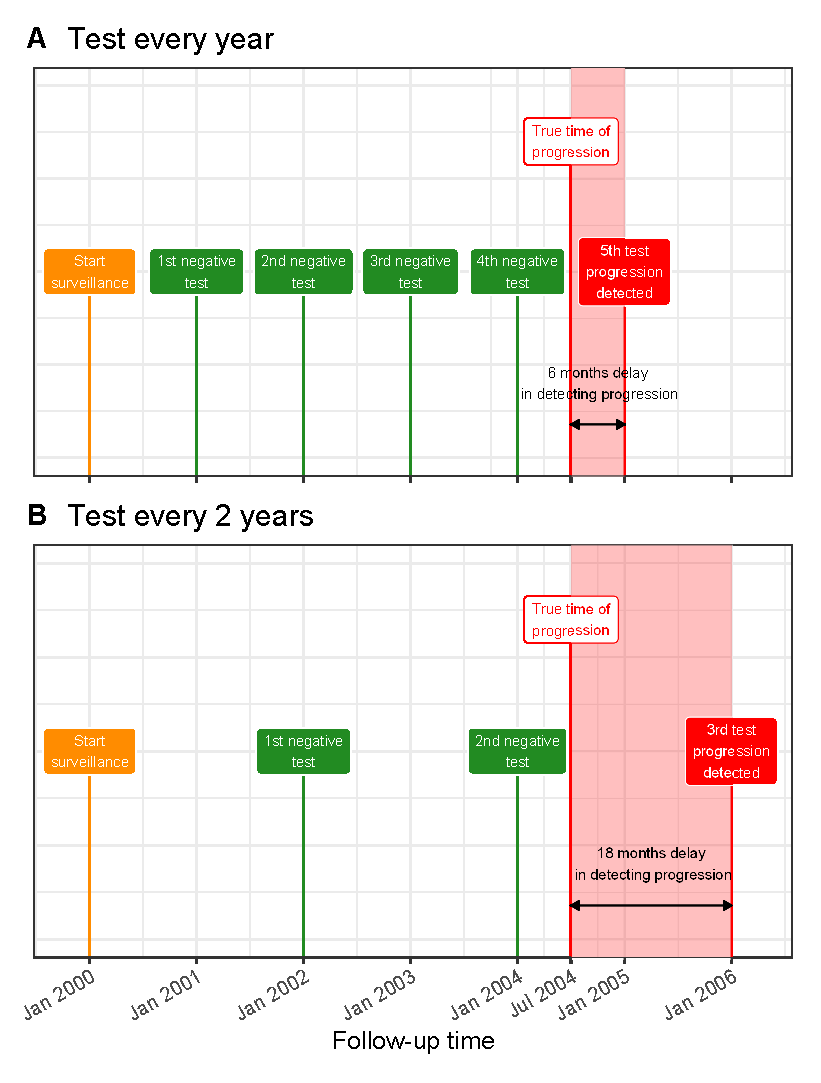
\includegraphics{images/delay_explanation.eps}}
\caption{\textbf{Trade-off between the number of invasive tests and time delay in detecting progression (non-terminal event of interest):} The true time of progression for this patient July 2004. More frequent invasive tests in \textbf{Panel~A} lead to a smaller time delay in detecting progression than less frequent invasive tests in \textbf{Panel~B}. Since invasive tests are conducted periodically, the time of progression is observed as an interval. For example, between Jan~2004--Jan~2005 in \textbf{Panel~A} and between Jan~2004--Jan~2006 in \textbf{Panel~B}.} 
\label{fig:delay_explanation}
\end{figure}

In this paper, we aim to balance the number of invasive tests (burden) and the time delay in detecting disease progression (less is beneficial) better than fixed schedules. For this purpose, we intend to create personalized test schedules that exploit patient-specific clinical data accumulated during follow-up. In surveillance, this data includes baseline characteristics of patients; results from previous invasive tests; and auxiliary longitudinal outcomes such as biomarkers, physical examination, and medical imaging measurements, etc. Previous approaches for personalized schedules can be divided into three categories. First, heuristic methods such as decision making flowcharts, e.g.,~\citet{bokhorst2015compliance}. However, flowcharts discretize continuous clinical outcomes, often utilize only the last measurement, and ignore the measurement error in observed outcomes. The second method is employing partially observable Markov decision processes~\citep{alagoz2010operations, steimle2017markov} for personalized test decisions. Although, the curse of dimensionality limits their application with continuous longitudinal outcomes. Third, personalized schedules obtained by optimizing an explicit utility function of the clinical parameters of interest~\citep{bebu2017optimal,rizopoulos2015personalized}, including our previous work on scheduling biopsies in prostate cancer~\citep{tomer2019personalized}. In this work, we will employ the third approach.

Our methodology is as follows. First, we develop a full specification of the joint distribution of disease and patient-specific longitudinal outcomes and the time of \textit{progression}. We achieve this using joint models for time-to-event and longitudinal data~\citep{tsiatis2004joint,rizopoulos2012joint}. We use joint models because they are inherently personalized. Specifically, they exploit patient-specific random effects~\citep{laird1982random} to model longitudinal outcomes without discretizing them. We subsequently employ the fitted joint model for new patients to estimate their patient-specific cumulative-risk of progression over their current and future follow-up visits. These risk predictions utilize their clinical data accumulated until their latest follow-up. We schedule invasive tests on all those future time points where a patient's conditional cumulative-risk of progression is equal to a certain threshold (e.g., 10\% risk). We then automate the choice of this threshold and the resulting schedule. More specifically, we optimize a function of the number of tests in a schedule and the expected time delay in detecting progression (Figure~\ref{fig:delay_explanation}). We estimate this time delay in a patient-specific manner for both fixed and personalized schedules. This can help patients/doctors to evaluate the consequences of opting for personalized versus fixed schedules objectively.

This research is motivated by the problem of scheduling biopsies~\citep{nieboer2018active} in the world's largest prostate cancer active surveillance study PRIAS~\citep{bokhorst2015compliance}. It has 7813 patients, 104,904 longitudinal measurements, and 1134 patients with cancer progression. These patients have low/very-low grade prostate cancer, often over-diagnosed due to prostate-specific antigen (PSA) based screening tests~\citep{crawford2003epidemiology}. The goal of surveillance upon diagnosis is to delay serious treatments (e.g., surgery, chemotherapy, etc.) until cancer progresses further. For this purpose, patients are monitored continually via PSA (ng/mL) blood tests, digital rectal examination (DRE) for shape and size of the tumor, and biopsy Gleason grade group~\citep{epsteinGG2014}. Since biopsy results are the strongest indicator of cancer-related outcomes, treatment is commonly advised upon observing an increase in a patient's biopsy Gleason grade group (cancer progression). The most commonly used schedule of biopsies in prostate cancer active surveillance is annual biopsies~\citep{loeb2014heterogeneity}. However, they lead to many unnecessary biopsies in slow/non-progressing patients (50\% proportion in some cohorts). Biopsy burden combined with patient non-compliance to frequent biopsies~\citep{bokhorst2015compliance} has raised concerns regarding the optimal biopsy schedule. Since prostate cancer has the second-highest incidence among all cancers in males~\citep{GlobalCancerStats2012}, biopsy schedules tailored for individual patients can reduce the overall burden of biopsies in a large number of patients worldwide.

The rest of the paper is as follows. Section~\ref{sec:jointmodel} briefly introduces the joint modeling framework. In Section~\ref{sec:schedule}, we present the methodology for personalized schedules and then demonstrate them for biopsies in real PRIAS patients in Section~\ref{sec:results}. Lastly, in Section~\ref{sec:sim_study}, we show the efficacy of personalized schedules via a realistic simulation study based on PRIAS patients.